\section{Spatial Attention: A Scheduling Hypothesis}
\label{sec:analysis}
\textbf{Measurements.} We measure prefill attention on ScanQA~\citep{azuma2022scanqa} validation using LLaVA-3D-7B and 3D-LLaVA-7B-LoRA. The former uses roughly 1500 image-derived spatial tokens from 20 views; the latter uses 100 superpoint tokens. The original profiles cover 50 distinct scenes per model. Expanded profiles use 200 questions from 67 scenes for LLaVA-3D and one question from each of 71 scenes for 3D-LLaVA. Let $\mathbf{A}^{(\ell)}$ be head-averaged attention, $g$ the last prompt position, $\mathcal{S}$ the spatial span, and $S^{(\ell)}=\sum_{j\in\mathcal{S}}\mathbf{A}^{(\ell)}_{g,j}$. We measure the spatial attention mass and the fraction of spatial tokens needed to cover $p=0.5,0.9$ of that mass:
\begin{align}
\alpha^{(\ell)} &= S^{(\ell)}\Big/\!\textstyle\sum_{j}\mathbf{A}^{(\ell)}_{g,j}, \\[-1pt]
C^{(\ell)}_{p} &= \frac{1}{|\mathcal{S}|}\min\!\big\{k:\textstyle\sum_{j\in\mathcal{T}^{(\ell)}_{k}}\mathbf{A}^{(\ell)}_{g,j}\ge p\,S^{(\ell)}\big\},
\end{align}
where $\mathcal{T}^{(\ell)}_k$ contains the top-$k$ spatial keys. \Cref{fig:threephase}(c) instead measures received-attention inequality across spatial keys. Let $T$ denote the total prompt length, including spatial and text tokens. For $N=|\mathcal{S}|$, define $r_j^{(\ell)}=\sum_{q=0}^{T-1}\mathbf{A}^{(\ell)}_{q,j}$ and sort these values in ascending order as $r_{(i)}^{(\ell)}$. We compute
\begin{equation}
G^{(\ell)}=
\frac{\sum_{i=1}^{N}(2i-N-1)r_{(i)}^{(\ell)}}
{N\sum_{i=1}^{N}r_{(i)}^{(\ell)}+10^{-9}}.
\end{equation}
The sum includes all prefill query positions, whereas attention mass and coverage use only the last prompt. We first average attention over heads, compute each statistic per sample, and then average it per layer.

\begin{figure*}[t]
\centering
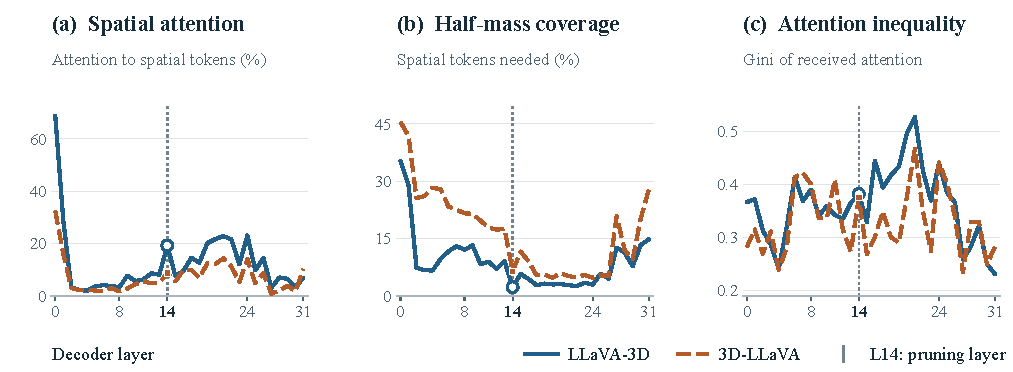
\includegraphics[width=\textwidth]{fig1_three_phase.pdf}
\caption{\textbf{Spatial attention across decoder layers, averaged over 50 scenes per model.} From L13 to L14, the last prompt token assigns more attention to spatial tokens (a), while fewer of them account for half of that spatial attention (b). Panel~(c) shows the Gini coefficient of attention received by spatial tokens from all prompt positions. Markers identify the selected pruning layer, L14. The curves show aggregate values; intervals for the expanded profiles are reported in the text.}
\label{fig:threephase}
\end{figure*}

\textbf{A concentrated late resurgence.} \Cref{fig:threephase} shows broad early access (L0--1), low direct spatial attention (L2--13), concentrated renewed access (L14--26), and a more diffuse tail (L27--31). These layer ranges describe the observed attention pattern without establishing stages of internal scene reasoning. The expanded profiles show late-phase spatial attention of 15.2\% $[14.3,16.1]$ for LLaVA-3D and 9.7\% $[8.7,10.7]$ for 3D-LLaVA. Their half-mass coverages are 4.0\% $[3.7,4.2]$ and 5.8\% $[5.2,6.4]$, corresponding to about 56 and 6 tokens. Bounds are scene-clustered 95\% bootstrap intervals for the expanded profiles.

\textbf{Stability across profiles and prompts.} For LLaVA-3D and 3D-LLaVA, respectively, late-minus-middle mean attention differences are 10.53 points $[9.71,11.34]$ and 6.52 points $[5.59,7.44]$. The corresponding L14--L13 jumps are 10.60 $[9.82,11.38]$ and 4.17 $[3.38,5.00]$. The L14 jump remains positive when we remove or paraphrase the answer suffix. A label-free onset rule also selects L14 across scene refits. Its window and threshold were chosen after profile inspection, so this checks stability without independently validating the rule. Both backbones are Llama-family 7B models; representation and training differences preclude controlled scaling or cross-backbone conclusions.

These profiles motivate testing late pruning through selected-set relevance and retention quality. They cannot resolve semantic identity, attention sinks, individual-token causality, or the decoding mechanism.
